\documentclass[a4paper,10pt]{article}
\usepackage[T1]{fontenc}
\usepackage[utf8]{inputenc}
\usepackage[english]{babel}
\usepackage{lmodern}
\usepackage[top=1.6cm,bottom=1.8cm,left=1.9cm,right=1.9cm]{geometry}
\usepackage{titlesec,enumitem,xcolor,graphicx,lastpage,fancyhdr}
\usepackage{fontawesome5}
\usepackage[hidelinks]{hyperref}

\hypersetup{colorlinks=true,urlcolor=blue!70!black,linkcolor=blue!70!black}
\pagestyle{fancy}\fancyhf{}\renewcommand{\headrulewidth}{0pt}
\fancyfoot[C]{\small\color{gray}Page \thepage\ of \pageref{LastPage}}
\setlength{\parindent}{0pt}

\titleformat{\section}{\large\bfseries\color{blue!70!black}}{}{0em}{}[\vspace{-0.7em}\rule{\textwidth}{0.5pt}]
\titlespacing{\section}{0pt}{9pt}{5pt}
\setlist[itemize]{leftmargin=1.1em,itemsep=2pt,topsep=2pt,parsep=0pt}
\newcommand{\role}[4]{\vspace{3pt}\noindent\hspace{0.6em}\parbox[t]{0.38\textwidth}{\raggedright\textbf{#1}}\hfill\parbox[t]{0.58\textwidth}{\raggedleft\textit{#2}}\\{\textit{#3}\hfill\textit{#4}}\vspace{1pt}}

\begin{document}
\noindent
\begin{minipage}[t]{0.78\textwidth}
\vspace{0pt}
{\huge\bfseries Prabhavit Gupta}\\[8pt]
{\small \faPhone\ +39-351-610-7807 \quad \faEnvelope\ \href{mailto:prabhavitg@gmail.com}{prabhavitg@gmail.com} \quad \faLinkedin\ \href{https://www.linkedin.com/in/prabhavit/}{Linkedin} \quad \faMapMarker*\ Venice, Italy}
\end{minipage}\hfill
\begin{minipage}[t]{0.18\textwidth}
\vspace{0pt}\raggedleft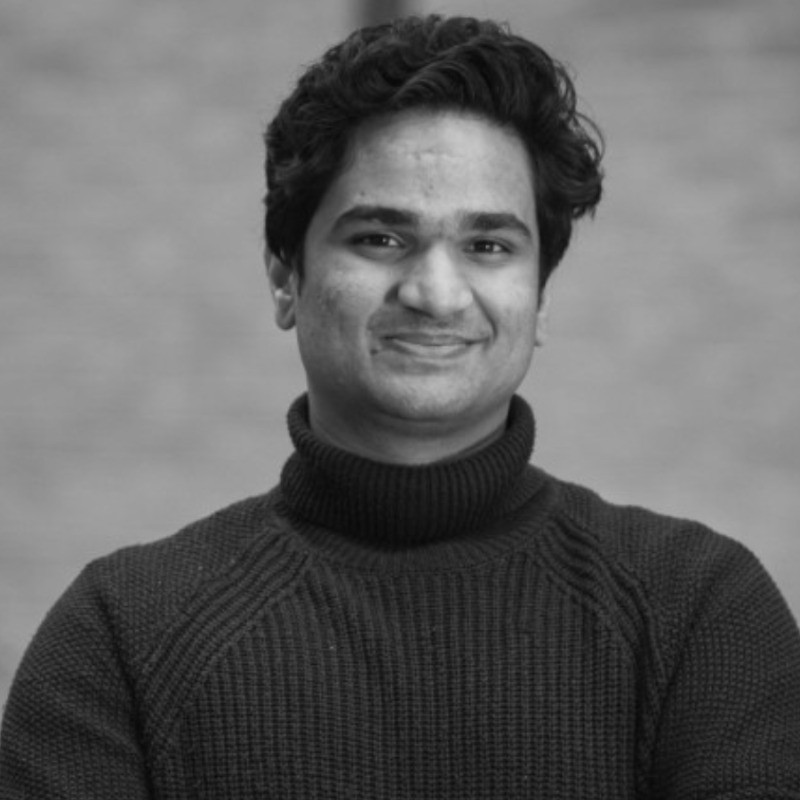
\includegraphics[width=2.3cm,height=2.3cm,keepaspectratio]{photo.jpg}
\end{minipage}

\section{Career Summary}
\begin{itemize}
\item Automation Software Engineer holding dual degrees in Mechanical Engineering (B.E.) and Management Engineering (M.Sc., Politecnico di Milano).
\item Solid foundation in programming, optimizing, and debugging PLC software for automated machinery across Siemens (TIA Portal) and Rockwell Automation platforms.
\item Hands-on expertise interfacing field hardware including brushless motors, servo-drives, optical/inductive sensors, and pneumatic actuators with control logic.
\item Experienced in electrical schematic interpretation, hardware-in-the-loop diagnostic testing, factory collaudo, and site commissioning.
\end{itemize}

\section{Technical Skills}
\begin{itemize}
\item \textbf{PLC Programming Platforms} -- Siemens TIA Portal (S7-1200, S7-1500), Rockwell Automation / Allen-Bradley (Studio 5000 / RSLogix), Ladder (LAD), Structured Text (SCL)
\item \textbf{Motion Control \& Field Devices} -- Servo Drives, Frequency Inverters, Stepper Motors, Encoders, Pneumatic Actuators, Industrial Sensors (Photoelectric, Proximity)
\item \textbf{Industrial Communication} -- PROFINET, PROFIBUS, Ethernet/IP, Modbus TCP/RTU, OPC UA, Fieldbus Couplers
\item \textbf{Testing, Collaudo \& Debugging} -- FAT/SAT Protocols, Software Fault Isolation, Machine Commissioning, Root Cause Analysis, Electrical Schematics
\item \textbf{Software \& Tools} -- Python, C++, Bash, SQL, Git, Linux, Technical Documentation
\end{itemize}

\section{Visa \& Language}
\begin{itemize}
\item \textbf{Language} -- Italian (Conversational / Intermediate), English (Fluent / Professional), Hindi (Native)
\item \textbf{Work Authorization} -- European Long Term Residence Permit (No Visa Sponsorship required). Driving License (Patente B). Available for on-site role in Milan.
\end{itemize}

\section{Professional Experience}
\role{\href{https://flowspace.co}{FlowSpace.co}}{Automation Software \& Systems Lead}{London, UK / Remote}{Mar 2024 -- Ongoing}
\begin{itemize}
\item \textbf{Control Software Development \& Optimization:}
\begin{itemize}[label=--]
\item Architected automated process control routines and continuous diagnostic suites for distributed machinery interfaces.
\item Developed high-speed telemetry handlers in Python and C++ monitoring drive response times, cycle parameters, and error states.
\item Authored technical machine specifications, functional descriptions, and debugging procedures for field engineers.
\end{itemize}
\item \textbf{Hardware-Software Integration:}
\begin{itemize}[label=--]
\item Coordinated multi-protocol communication bridges interfacing field sensors and actuators with central supervisory logic.
\item Maintained 99.9\% machine operational availability through proactive fault isolation and software logic refactoring.
\end{itemize}
\item \textit{Tools: Python, C++, Linux, Modbus, Industrial Networks, Docker, Git}
\end{itemize}

\role{Urlink}{Systems Automation Engineer}{Milan, Italy}{Jul 2023 -- Feb 2024}
\begin{itemize}
\item Conducted on-site machine testing, electrical schematic verification, and PLC program debugging during system collaudo.
\item Configured servo-drive motion parameters, safety interlocks, and sensor inputs according to functional project specifications.
\item Partnered with electrical engineering teams to resolve field wiring and communication anomalies during final commissioning.
\end{itemize}

\role{UltraStrategy}{Automation Developer}{Remote, Germany}{Sep 2022 -- Jun 2023}
\begin{itemize}
\item Developed automated scripts collecting machine operational data, cycle throughput, and diagnostic error codes.
\item Structured equipment performance telemetry into comprehensive technical reports for quality assurance reviews.
\end{itemize}

\section{Education}
\role{Politecnico di Milano}{M.Sc. in Management Engineering (Digital Business \& ICT)}{Milan, Italy}{2020 -- 2023}
\role{Thapar Institute of Engineering and Technology}{B.E. in Mechanical Engineering}{Punjab, India}{2014 -- 2018}

\end{document}
